\chapter{Teknik \textit{Dynamic Programming}}\label{ch:modul5}

\section{Pengenalan \textit{Dynamic Programming}}
\textit{Dynamic programming} merupakan pendekatan lain dalam memecahkan permasalahan seperti pendekatan \textit{divide and conguer}. Kata \textit{programming} di nama \textit{dynamic programming} tidak berhubungan dengan menulis kode komputer melainkan lebih ke arah metode tabular (kata \textit{dynamic programming} sebenarnya dipopulerkan di bidang matematika bukan ilmu komputer/teknik informatika).

Di \textit{divide and conguer}, permasalahan dipecah menjadi sub-permasalahan yang lebih kecil kemudian dipecahkan secara terpisah dan akhirnya digabungkan. Kelemahan dalam pendekatan ini adalah, beberapa sub-permasalahan sebenarnya memiliki solusi pemecahan yang sama akan tetapi di \textit{divide and conguer} hal itu tidak diperdulikan, melainkan sub-permasalahan yang sama akan diselesaikan berkali-kali sehingga mengakibatkan pemborosan sumber daya komputasional.

Di \textit{dynamic programming} sub-permasalahan yang sama hanya dipecahkan sekali saja dan disimpan solusinya ke dalam tabel (itu sebabnya ia disebut sebagai metode tabular). Apabila ditemukan sub-permasalahan yang sama kelak, maka solusi yang telah disimpan akan dipergunakan kembali.

\textit{Dynamic programming} sering dipakai untuk menyelesaikan permasalahan yang bersifat optimisasi. Permasalahan tersebut mempunyai berbagai macam solusi, akan tetapi hanya ada satu yang nilainya optimal (misalnya nilai paling maksimal atau minimal). Nilai yang paling optimal tersebut disebut juga sebagai solusi optimal dari suatu permasalahan.

Terdapat 4 langkah dalam penyelesaian permasalahan \textit{dynamic programming}:
\begin{enumerate}
	\item Gambarkan struktur dari solusi optimal.
	\item Definisikan nilai dari solusi optimal secara rekursif.
	\item Hitung nilai dari solusi optimal.
	\item Bentuk solusi optimal dari informasi yang sudah dihitung sebelumnya.
\end{enumerate}

\section{Contoh DP: Pemotongan Rotan}
Sebagai salah satu contoh permasalahan yang bisa diselesaikan dengan menggunakan \textit{dynamic programming}, kita akan menyelesaikan permasalahan pemotongan rotan. 

Sebuah perusahaan membeli berbagai rotan dengan panjang berbeda-beda. Rotan tersebut akan dipotong menjadi beberapa rotan yang lebih pendek kemudian akan dijual lagi. Untuk setiap pemotongan tidak dikenakan biaya. Pihak manajemen dari perusahaan tersebut ingin mengetahui cara paling optimal untuk memotong rotan-rotan tersebut.

Asumsi kita mengetahui untuk setiap nilai $i=1,2,\ldots,$ $p_i$ merupakan harga yang ditetapkan perusahaan tersebut ketika menjual rotan dengan panjang $i$ inci. Panjang dari rotan akan selalu dalam bentuk integer. 

Definisi formal dari permasalahan tersebut adalah sebagai berikut.

\begin{contoh}
\textbf{Permasalahan Pemotongan Rotan}\\
Diketahui sebuah rotan dengan panjang $n$ dan sebuah tabel harga $p_i$ untuk $i=1,2,\ldots,n$, tentukan keuntungan maksimum $r_n$ yang bisa diperoleh dengan memotong rotan menjadi rotan-rotan yang lebih pendek. \\
\textbf{Masukan:}\\
Sebuah \textit{array} $p_i$ dimana $i=1,2,..,n$ dan $p_i$ adalah harga untuk panjang $i$.\\
\textbf{Keluaran:}\\
Sebuah nilai $r_n$ yang merupakan nilai optimal dari pemotongan rotan $n$ dan kemudian dijual. Ada juga kemungkinan rotan tak perlu dipotong tetapi sudah memiliki harga yang tinggi daripada harus dipotong lagi.\\
\end{contoh}

\begin{figure}[H]%
\centering
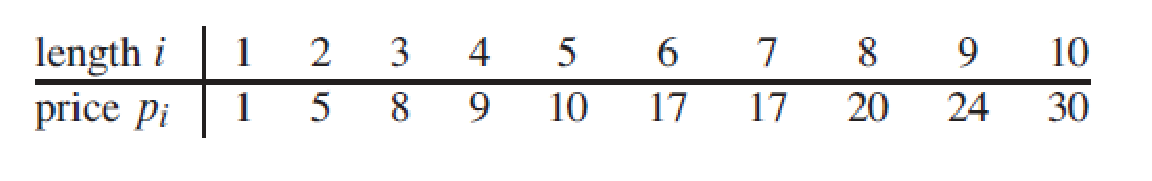
\includegraphics[scale=0.6]{fig/rodCutting.eps}%
\caption{Perbandingan panjang $p_i$ dan harga $i$}%
\label{fig:rodCutting}%
\end{figure}

Sebagai contohnya, ketika $n=4$, sesuai dengan tabel di Gambar \ref{fig:rodCutting} maka jika rotan tidak dipotong ($n=4$) harganya $p_4 = 9$ sedangkan jika dipotong menjadi 2 bagian yang sama panjang ($n=2$) maka harganya menjadi $r_4=p_2+p_2=5+5=10$ yang merupakan nilai optimal (lihat Gambar \ref{fig:rodCutting2}).   

\begin{figure}[H]%
\centering
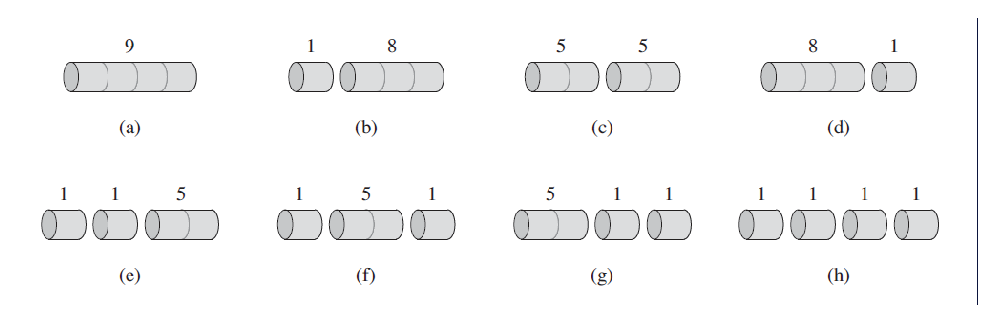
\includegraphics[scale=0.7]{fig/rodCutting2.eps}%
\caption{Berbagai jenis potongan yang mungkin. Potongan yang paling optimal adalah yang bagian (c).}%
\label{fig:rodCutting2}%
\end{figure}

Dengan observasi dan nilai $n$ yang kecil kita bisa menentukan nilai optimal untuk setiap ukuran sebagai berikut. \\
r1 = 1 dari solusi 1 = 1 (tidak potong) ;\\
r2 = 5 dari solusi 2 = 2 (tidak potong) ;\\
r3 = 8 dari solusi 3 = 3 (tidak potong) ;\\
r4 = 10 dari solusi 4 = 2 + 2 ;\\
r5 = 13 dari solusi 5 = 2 + 3 ;\\
r6 = 17 dari solusi 6 = 6 (tidak potong) ;\\
r7 = 18 dari solusi 7 = 1 + 6 or 7 = 2 + 2 + 3 ;\\
r8 = 22 dari solusi 8 = 2 + 6 ;\\
r9 = 25 dari solusi 9 = 3 + 6 ;\\
r10 = 30 dari solusi 10 = 10 (tidak potong).

Banyaknya kemungkinan cara yang ada untuk memotong rotan $n$ adalah $2^{n-1}$ cara yang berbeda. Nilai $2^{n-1}$ didapat melalui perhitungan dimana setiap nilai $i$ sampai $n-1$ (jika panjang $n$ maka ada $n-1$ tempat untuk dipotong) ada 2 kemungkinan yang ada yaitu potong atau tidak potong. Jadi, untuk $n=4$ maka jumlah kemungkinannya adalah $2\times{}2\times{}2 = 8$ atau $2^3$. 

Solusi penyelesaian pemotongan rotan dengan menggunakan algoritma naive rekursif adalah sebagai berikut.

\begin{algorithm}[H]
	\caption{CUT-ROD-NAIVE($p,n$)}
	\label{algo:cutRodNaive}
	\begin{algorithmic}[1]
		\IF{$n == 0$}
			\RETURN 0
		\ENDIF
		\STATE $q=-\infty$
		\FOR{$i$ \TO $n$}
			\STATE $q= max(q, p[i] + $CUT-ROD-NAIVE$(p,n-i))$
		\ENDFOR
	\end{algorithmic}
\end{algorithm}

Sedangkan solusi penyelesaian dengan menggunakan metode \textit{Dynamic Programming} ada dua macam penyelesaian yaitu \textit{Bottom Up} dan \textit{Top Down}.

\begin{algorithm}[H]
	\caption{MEMOIZED-CUT-ROD($p,n$)}
	\label{algo:memoizedCutRod}
	\begin{algorithmic}[1]
		\STATE let $r[0..n]$ be a new array
		\FOR{$i$ \TO $n$}
			\STATE $r[i]=-\infty$
		\ENDFOR
		\RETURN MEMOIZED-CUT-ROD-AUX($p,n,r$)
	\end{algorithmic}
\end{algorithm}

\begin{algorithm}[H]
	\caption{MEMOIZED-CUT-ROD-AUX($p,n,r$)}
	\label{algo:memoizedCutRodAux}
	\begin{algorithmic}[1]
		\IF{$r[n]\geq 0$}
			\RETURN $r[n]$
		\ENDIF
		\IF{$n==0$}
			\STATE $q=0$
		\ELSE
			\STATE $q=-\infty$
			\FOR{$i=1$ \TO $n$}
				\STATE $q=max(q,p[i]+$MEMOIZED-CUT-ROD-AUX$(p,n-1,r))$
			\ENDFOR
		\ENDIF
		\STATE $r[n]=q$
		\RETURN $q$
	\end{algorithmic}
\end{algorithm}

\begin{algorithm}[H]
	\caption{BOTTOM-UP-CUT-ROD($p,n$)}
	\label{algo:bottomUpCutRod}
	\begin{algorithmic}[1]
		\STATE let $r[0..n]$ be a new array
		\STATE $r[0] = 0$
		\FOR{$j=1$ \TO $n$}
			\STATE $q=-\infty$
			\FOR{$i=1$ \TO $j$}
				\STATE $q=max(q,p[i]+r[j-i])$
			\ENDFOR
			\STATE $r[j] = q$
		\ENDFOR
		\RETURN $r[n]$
	\end{algorithmic}
\end{algorithm}

Kita bisa menyempurnakan algoritma \ref{algo:bottomUpCutRod} supaya bisa menampilkan solusi dari setiap panjang optimal dari permasalahan pemotongan rotan dengan algoritma berikut.

\begin{algorithm}[H]
	\caption{EXTENDED-BOTTOM-UP-CUT-ROD($p,n$)}
	\label{algo:extBottomUpCutRod}
	\begin{algorithmic}[1]
		\STATE let $r[0..n]$ be a new array
		\STATE $r[0] = 0$
		\FOR{$j=1$ \TO $n$}
			\STATE $q=-\infty$
			\FOR{$i=1$ \TO $j$}
				\IF{$q<p[i]+r[j-i]$}
					\STATE $q=p[i]+r[j-i]$
					\STATE $s[j]=i$
				\ENDIF
			\ENDFOR
			\STATE $r[j] = q$
		\ENDFOR
		\RETURN $r[n]$
	\end{algorithmic}
\end{algorithm}

\begin{algorithm}[H]
	\caption{PRINT-CUT-ROD-SOLUTION($p,n$)}
	\label{algo:printCutRodSolution}
	\begin{algorithmic}[1]
		\STATE $(r,s)$ = EXTENDED-BOTTOM-UP-CUT-ROD($r,n$)
		\WHILE{$n>0$}
			\STATE print $s[n]$
			\STATE $n = n - s[n]$
		\ENDWHILE
	\end{algorithmic}
\end{algorithm}

\begin{figure}[H]%
\centering
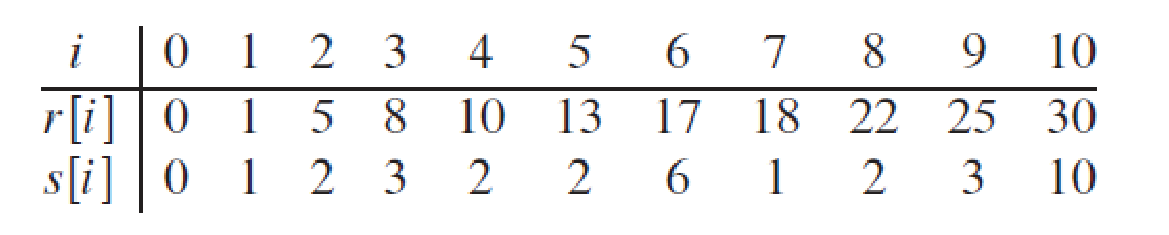
\includegraphics[scale=0.5]{fig/CutRodSolution.eps}%
\caption{Solusi dari permasalahan pemotongan rotan.}%
\label{fig:cutRodSolution}%
\end{figure}

\section{Contoh DP: Pengalian Rangkaian Matriks}

Salah satu permasalahan yang sangat umum di \textit{Dynamic Programming} adalah permasalahan pengalian rangkaian matriks. Dalam masalah ini diberikan sebuah rangkaian matriks $\left\langle A_{1},A_{2},\ldots,A_{n} \right\rangle$ yang terdiri dari $n$ matriks dimana akan dicari pengalian paling optimal dari rangkaian matriks.  

Jika seandainya terdapat 4 buah matriks dalam sebuah rangkaian $\left\langle A_{1},A_{2},A_{3},A_{4} \right\rangle$ maka kemungkinan yang terdapat untuk mengalikan matriks tersebut adalah sebagai berikut.


$(A_{1}(A_{2}(A_{3}A_{4})))$,\\
$(A_{1}((A_{2}A_{3})A_{4}))$,\\
$((A_{1}A_{2})(A_{3}A_{4}))$,\\
$((A_{1}(A_{2}A_{3}))A_{4})$,\\
$(((A_{1}A_{2})A_{3})A_{4})$.

Dari kelima kemungkinan cara pengalian diatas, setiap cara akan memiliki biaya pengalian yang berbeda. Untuk menyederhanakan, kita akan menggunakan 3 buah matriks dalam satu rangkaian $\left\langle A_{1},A_{2},A_{3} \right\rangle$ dengan dimensi dari setiap matriks dalam rangkaian tersebut adalah 10 X 100, 100 X 5 dan 5 X 50. 

Semisalnya kita mengalikan sesuai dengan cara $((A_{1}A_{2})A_{3})$ maka biaya yang diperlukan adalah 10.100.5 = 5000 sesuai dengan perkalian skalar untuk menghitung $A_{1}A_{2}$ ditambah 10.5.50 = 2500 untuk mengalikan hasilnya dengan $A_{3}$. Total dari semua adalah 5000+2500 = 7500.

Seandainya kita mengalikan dengan cara $(A_{1}(A_{2}A_{3}))$ maka perhitungan biayanya adalah: pengalian $A_{2}A_{3}$ sebesar 100.5.50 = 25000 ditambah dengan 10.100.50 = 50000 untuk mengalikan hasilnya dengan $A_{1}$. Total biaya adalah 25000+50000 = 75000. Dari dua cara pengalian bisa disimpulkan bahwa pengalian dengan cara pertama lebih efisien.

Berdasarkan illustrasi diatas, maka bisa permasalahan perkalian matriks bisa dituliskan sebagai berikut. Diberikan sebuah rangkaian $\left\langle A_{1},A_{2},\ldots,A_{n} \right\rangle$ dari $n$ matriks dimana $i=1,2,\ldots,n$ dan matriks $A_{i}$ memiliki dimensi $p_{i-1}xp_{i}$, carilah cara pengalian yang memiliki biaya perkalian skalar yang terkecil.

Secara matematis solusi dari permasalahan perkalian matriks bisa ditulis sebagai:

\begin{figure}[H]%
	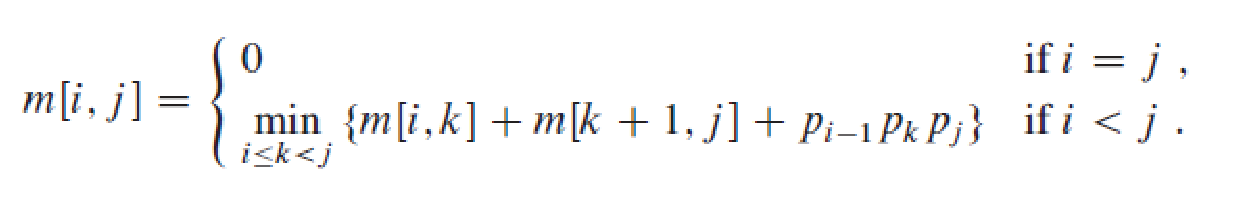
\includegraphics[scale=0.4]{fig/math-matrix.eps}%
	\label{fig:math-matrix}%
\end{figure}

Algoritma yang digunakan untuk mencari solusi optimal dari perkalian matriks adalah sebagai berikut.

\begin{algorithm}[H]
	\caption{MATRIX-CHAIN-ORDER($p$)}
	\label{algo:matrixChainOrder}
	\begin{algorithmic}[1]
		\STATE $n=p.length-1$
		\STATE let $m[1..n,1..n]$ and $s[1..n-1,2..n]$ be new tables
		\FOR{$i=1 $\TO$n$}
			\STATE $m[i,i] = 0$
		\ENDFOR
		\FOR{$l=2$ \TO$n$}
			\FOR{$i=1$ \TO$n-l+1$}
				\STATE $j=i+l-1$
				\STATE $m[i,j]=\infty$
				\FOR{$k=i$ \TO$j-1$}
					\STATE $q=m[i,k]+m[k+1,j]+p_{i-1}p_{k}p_{j}$
					\IF{$q<m[i,j]$}
						\STATE $m[i,j]=q$
						\STATE $s[i,j]=k$
					\ENDIF			
				\ENDFOR
			\ENDFOR
		\ENDFOR
		\RETURN $m$ and $s$
	\end{algorithmic}
\end{algorithm}

Dari Algoritma \ref{algo:matrixChainOrder} akan dihasilkan dua buah matriks yaitu tabel $m$ dan tabel$s$. Sebagai contoh, jika rangkaian matriks yang digunakan adalah sebagai berikut.

\begin{figure}[H]%
	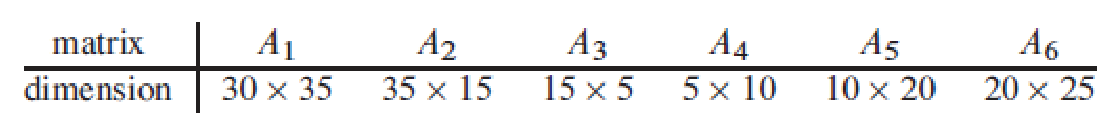
\includegraphics[scale=0.5]{fig/matrix.eps}%
	\label{fig:matrix}%
\end{figure}

maka tabel $m$ dan tabel $s$ yang diperoleh adalah:
\begin{figure}[H]%
	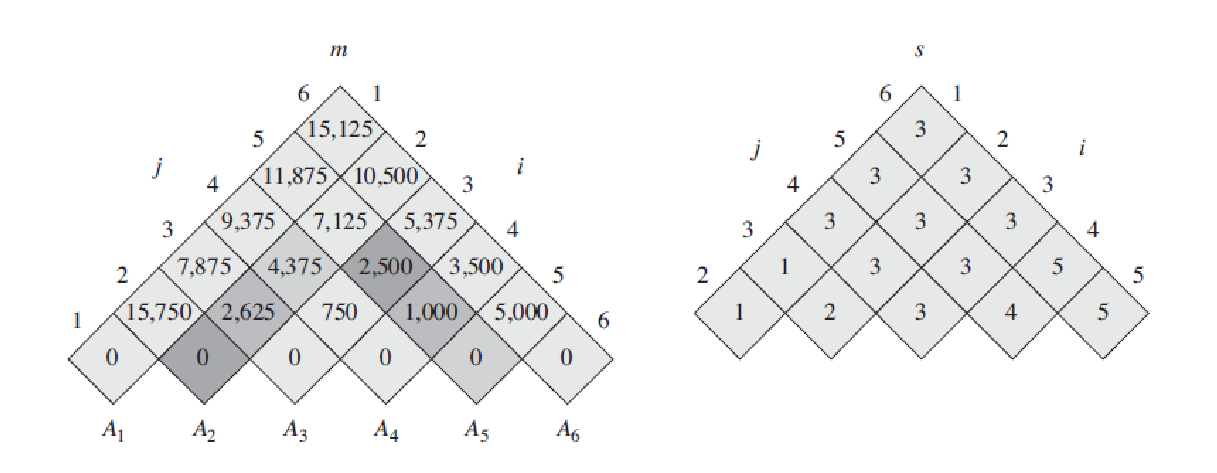
\includegraphics[scale=0.7]{fig/matrix2.eps}%
	\caption{Tabel $m$ dan $s$ yang diperoleh dengan jumlah matriks sebanyak 6 buah}
	\label{fig:matrix2}%
\end{figure}
